%% This documentation was generated with Faust version 2.0.a3
%% Fri May 27 13:32:07 2011
%% http://faust.grame.fr

\documentclass{article}

\usepackage[utf8]{inputenc}
\usepackage{graphicx}
\usepackage[usenames]{color}
\usepackage{listings}
\usepackage{supertabular}
\usepackage{amsmath}
\usepackage{latexsym, amssymb}
\usepackage{breqn}

% No indent
\setlength{\parindent}{0pt}

% Make LaTeX output a dot when typing an asterisk
\DeclareMathSymbol{*}{\mathbin}{symbols}{"01}

% lstlistings setup
\definecolor{yobg}{rgb}{0.9,0.9,1}
\definecolor{yotxt}{rgb}{0.01,0.01,0.52} % a dark blue.
\definecolor{mylstbg}{rgb}{0.98,0.98,0.98} % a really pale grey.
\definecolor{mylstcmt}{rgb}{0.01,0.52,0.01} % a dark green.
\definecolor{mylstdoc}{rgb}{0.80,0.30,0.80} % a medium pink.

\lstset{%
  language=C++, 
  numbers=left,%none,
  tabsize=4, 
  frame=single, 
  breaklines=true, 
  numberstyle=\tiny\ttfamily, 
  backgroundcolor=\color{mylstbg}, 
  basicstyle=\scriptsize\ttfamily, 
  commentstyle=\slshape\color{mylstcmt}, %\itshape,
  frameround=tttt, 
  columns=flexible, %fixed, 
  showstringspaces=false,
  emptylines=2,
  inputencoding=utf8,
  emph={component, declare, environment, import, library, process},
  emph={[2]ffunction, fconstant, fvariable},
  emph={[3]button, checkbox, vslider, hslider, nentry, vgroup, hgroup, tgroup, vbargraph, hbargraph, attach},
  emphstyle=\color{yotxt}, %\underline, %\bfseries,
  morecomment=[s][\color{mylstdoc}]{<mdoc>}{</mdoc>},
  rulecolor=\color{black}
}

\newcommand{\faustfilename}{testing/vol.dsp_generated.dsp}
\newcommand{\faustdocdir}{vol.dsp_generated-mdoc}
\newcommand{\faustprogname}{vol.dsp_generated}
\newcommand{\faustversion}{2.0.a3}
\newcommand{\faustdocdate}{May 27, 2011}

\begin{document}
\title{vol.dsp_generated}
\date{\today}
\maketitle

\bigskip
This document provides a mathematical description of the Faust program text stored in the \texttt{\faustfilename} file. See the notice in Section\,\ref{notice} (page\,\pageref{notice}) for details.


\section{Mathematical definition of \texttt{process}}
\label{equation}

The \emph{\faustprogname} program evaluates the signal transformer denoted by \texttt{process}, which is mathematically defined as follows:

% Set of Faust formulas (corresponding to an <equation> tag).
\begin{enumerate}

\item Output signals $y_i$ for $i \in [1,2]$ such that
	\begin{dgroup*}
		\begin{dmath*}
				y_{1}(t) = r_{1}(t)
		\end{dmath*}
		\begin{dmath*}
				y_{2}(t) = 0.5 * r_{1}(t)
		\end{dmath*}
	\end{dgroup*}

\item Input signal (none)

\item Intermediate signal  $r_1$ such that
	\begin{dgroup*}
		\begin{dmath*}
				r_{1}(t) = 1 \oplus r_{1}(t\!-\!1)
		\end{dmath*}
	\end{dgroup*}

\end{enumerate}


\section{Block diagram of \texttt{process}}
\label{diagram}

The block diagram of \texttt{process} is shown on Figure\,\ref{figure1} (page\,\pageref{figure1}).
\begin{figure}[ht!]
	\centering
	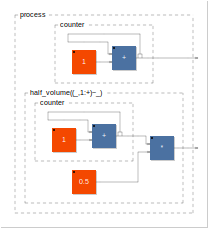
\includegraphics[width=\textwidth]{../svg/svg-01/process}
	\caption{Block diagram of \texttt{process}}
	\label{figure1}
\end{figure}


\section{Notice}
\label{notice}


\begin{itemize}
	\item This document was generated using Faust version \faustversion\ on \faustdocdate.
	\item The value of a Faust program is the result of applying the signal transformer denoted by the expression to which the \texttt{process} identifier is bound to input signals, running at the $f_S$ sampling frequency.
	\item Faust (\emph{Functional Audio Stream}) is a functional programming language designed for synchronous real-time signal processing and synthesis applications. A Faust program is a set of bindings of identifiers to expressions that denote signal transformers. A signal $s$ in $S$ is a function mapping\footnote{Faust assumes that $\forall \, s \in S, \forall \, t \in \mathbb{Z}, s(t) = 0 \mathrm{\ when\ } t < 0$.} times $t \in \mathbb{Z}$ to values $s(t) \in \mathbb{R}$, while a signal transformer is a function from $S^n$ to $S^m$, where $n,m\in \mathbb{N}$. See the Faust manual for additional information (\textsf{http://faust.grame.fr}).
	\item Every mathematical formula derived from a Faust expression is assumed, in this document, to having been normalized (in an implementation-depen\-dent manner) by the Faust compiler.
	\item A block diagram is a graphical representation of the Faust binding of an identifier I to an expression E; each graph is put in a box labeled by I. Subexpressions of E are recursively displayed as long as the whole picture fits in one page.
	\item 
		This document uses the following integer operations:
	\begin{center}
	\begin{tabular}{|c|l|l|} 
		\hline 
		\emph{operation} & \emph{name} & \emph{semantics} \\
		\hline 
		$i \oplus j$ & integer addition & $\mathrm{normalize}(i+j), \mathrm{~in~} \mathbb{Z}$ \\
		\hline 
	\end{tabular} 
	\end{center}
		Integer operations in Faust are inspired by the semantics of operations on the n-bit two's complement representation of integer numbers; they are internal composition laws on the subset $[\,-2^{n-1}, 2^{n-1}\!-\!1\,]$ of $\mathbb{Z}$, with $n = 32$. For any integer binary operation $\times$ on $\mathbb{Z}$, the $\otimes$ operation is defined as: $i \otimes j = \mathrm{normalize}(i \times j)$, with 
$$\mathrm{normalize}(i) = i - N\cdot\mathrm{sign}(i) \cdot \left\lfloor \frac{|i|+N/2+(\mathrm{sign}(i)\!-\!1)/2}{N} \right\rfloor , $$
 where $N = 2^n$ and $\mathrm{sign}(i) = 0 \mathrm{\ if\ } i=0 \mathrm{\ and\ } i / |i| \mathrm{\ otherwise}.$
Unary integer operations are defined likewise.
	\item The \texttt{\faustdocdir/} directory may also include the following subdirectories:
\begin{itemize}
	\item	\texttt{cpp/} for Faust compiled code; 
	\item	\texttt{pdf/} which contains this document; 
	\item	\texttt{src/} for all Faust sources used (even libraries); 
	\item	\texttt{svg/} for block diagrams, encoded using the Scalable Vector Graphics format (\textsf{http://www.w3.org/Graphics/SVG/});
	\item	\texttt{tex/} for the \LaTeX\ source of this document.
\end{itemize}
\end{itemize}


\section{Faust code listing}
\label{listing}

This section provides the listing of the Faust code used to generate this document.

\bigskip\bigskip
\begin{lstlisting}[caption=\texttt{vol.dsp_generated.dsp}]
if__(a,(k1,k2),(k3,k4)) = if__(a,k1,k3),if__(a,k2,k4);
if__(a,k,k)             = k;
if__(a,k1,k2)           = select2(a,k2,k1);


c___Vol__process(volume, input_1, retsel__) = 
  func__1925(volume, input_1, retsel__) with{
    func__1925(volume, input_1, retsel__) = 
      func__1926(volume, float(input_1), retsel__);

    func__1926(volume, input_1, retsel__) = 
      (volume, input_1, 0);

  };
c___Vol__process__return__(volume, input_1, retsel__) = 
      (input_1 * volume ) with{
  
};

c___Vol_____initrepeat(volume, input_1, retsel__) = 
  func__1927(volume, input_1, retsel__) with{
    func__1927(volume, input_1, retsel__) = 
      func__1928(float(volume), input_1, retsel__);

    func__1928(volume, input_1, retsel__) = 
      (volume, input_1, retsel__);

  };

c___Vol_____init(volume, input_1, retsel__) = 
  func__1929(volume, input_1, retsel__) with{
    func__1929(volume, input_1, retsel__) = 
      func__1930(float(volume), input_1, retsel__);

    func__1930(volume, input_1, retsel__) = 
      (volume, input_1, retsel__);

  };

c___Vol(volume, input_1) = (input_1 * volume );

half_volume = c___Vol ( 0.5 ) ; 
counter = + ( 1 ) ~ _ ; 
process = counter , half_volume ( counter ) ; 
                         
\end{lstlisting}


\end{document}

